\section{Teoría de Juegos / Interacciones sociales}
\econ{https://www.core-econ.org/the-economy/book/es/text/04.html}{4}
\newline
\newline
\textit{La Teoría de Juegos es una forma de entender cómo interactúan las personas basándose en las restricciones que limitan su actuar, sus motivaciones y sus creencias sobre el comportamiento de otras personas.}
\subsection{Juego}

Este consiste en distintos parámetros, los cuales son:
\begin{itemize}
    \item \textbf{Jugadores} (I)
    \item \textbf{Estrategias} (s): el conjunto (o perfil) de estrategias del jugador \textit{i} se denota por $S_i$ y una estrategia específica por $s_i$.
    \item \textbf{Función de pago o utilidad}: es dependiente de la estrategia escogida
\end{itemize}

Los juegos a considerar son los simultáneos o estáticos. Estos se pueden representar por una matriz de pago si hay 2 jugadores, y en la matriz se logra visualizar los jugadores, estrategias y pagos.

\begin{figure}[H]
    \centering
    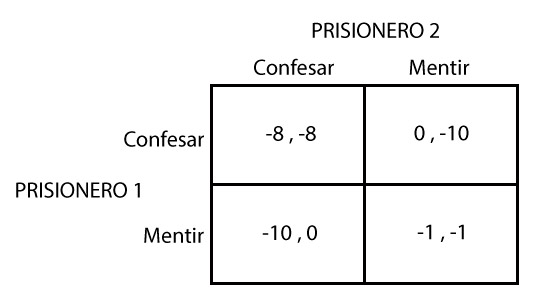
\includegraphics[width=0.5\textwidth]{Modulo_3/Dilema-del-prisionero.jpg}
    \caption{Matriz de juego del dilema del prisionero, donde las estrategias son: Confesar o Mentir y los pagos son los números mostrados en la casilla. El número de la izquierda corresponde al pago del prisionero 1 y el de la derecha al del 2.}
    \label{img:matriz-dilema-prisionero}
\end{figure}


El dilema mostrado en la Figura \ref{img:matriz-dilema-prisionero}, trata sobre dos prisioneros que les dan la opción de o confesar o de negar un crimen cometido por ambos. Y, según lo que escoge cada uno se definen los años que han de pasar en la cárcel. Por ejemplo, si ambos confiesan, irían ambos 8 años a la cárcel, y si uno miente y el otro confiesa, el mentiroso iría 10 años a la cárcel y el otro 0.

\subsection{Estrategias estrictamente dominadas (EED)}

Los juegos pueden tener estrategias EED, que equivale a que conviene siempre \textbf{no} usar esa estrategia (o usar otra) ya que el pago o utilidad de las demás es siempre mayor.

Diremos que $s_i \in S_i$ es una estrategia estrictamente dominada para el jugador \textit{i}, si existe otra estrategia $s_i' \in S_i$ tal que:
\[U_i(s_i', s_{-i}) > U_i(s_i, s_{-i}) \quad \forall s_{-i} \in S_{-i} \]

Aquí \textit{-i} hace referencia al resto de los jugadores y $U_i$ a la utilidad del jugador \textit{i} dada cierta estrategia.
\\
Las EED pueden ser utilizadas para predecir el resultado de juegos, ya que no es racional usar esas estrategias.

\subsection{Eliminación iterada de EEDs (EIEED)}

\textit{Permite, en algunos casos, resolver el juego. Aunque no necesariamente llevará a la solución óptima.}


La EIEED consiste en, como dice el nombre, eliminar iterativamente las EEDs de cada jugador. Dándose la posibilidad de que en cada paso puedan surgir nuevas EEDs de otros jugadores que también serán eliminadas, siguiendo así hasta que ya no queden más EEDs.

El supuesto de esto es la \underline{racionalidad compartida}: los jugadores no solo son racionales, también saben que los otros jugadores son racionales y viceversa. 
\\[0.2em]

En el caso del dilema del prisionero (Fig \ref{img:matriz-dilema-prisionero}) se tendrá por EIEED que la estrategia dominante será (Confesar, Confesar), obteniendo ambos 8 años de cárcel. 

\subsection{Equilibrio de Nash (EN)}

En el equilibrio, los jugadores no tienen incentivos a desviarse a otra estrategia. 

Un perfil de estrategias $s^* = (s^*_1, ..., s^*_N)$ es un EN si:
\[\forall i \in I, \forall s_i \in S_i \quad U_i(s^*_i, s^*_{-i}) \geq U_i(s_i, s^*_{-i})\]

En otras palabras, en un EN cada jugador está jugando su mejor estrategia dada la estrategias del otro. 

La mejor respuesta de un jugador en un determinado juego es la estrategia que maximiza su pago condicional a lo que están haciendo el resto de los jugadores.

%\subsubsectionanum{Caracterización de los EN}
%\[S^* es\\un\\EN \iff \forall i \in I: s^*_i \in BR_i(S^*_{-i})\]

\subsubsection{Características del EN}

\begin{itemize}
    \item El EN no necesariamente es óptimo para el conjunto de jugadores
    \item Se auto-sustenta, ningún jugador tiene incentivos a desviarse unilateralmente del equilibrio, i.e. no requiere de un jugador externo para sostenerse. 
    \item Si se juega muchas veces se llega a un EN
    \item Los jugadores racionales juegan $"$a la Nash$"$ (van siempre al equilibrio)
    \item Todo EN sobrevive a un EIEED
    \item Si el proceso EIEED finaliza con un único perfil, este es EN.
    \item Que un perfil sea EN $\iff$ a que todos los jugadores estén jugando su mejor respuesta a dicho perfil (mayor utilidad).
    \item De haber más de un equilibrio de Nash, no se sabe realmente cual se irá a escoger.
\end{itemize}

\subsection{Otros términos}

\subsubsection{Preferencias altruistas} Aportar más o ir por la opción que no necesariamente te beneficia a ti un 100\%, aumentando la ganancia del otro. Es como hacer el bien sin esperar que el otro también lo haga.


\subsubsection{Free rider} Polizones que se aprovechan de el altruismo o coordinación de los demas para obtener una ganancia sin aportar.


\subsubsection{Tragedia de los comunes} Como los pagos para los polizones dependen de la contribución total al bien público, la única forma de castigar a los free riders en los experimentos es dejar de contribuir. De haber otra forma de castigarlos se usa, pero puede traer resultados inesperados.


\subsubsection{Juego secuencial} Primero juega un jugador y en base a eso juega el otro.


\subsubsection{Juego simultáneo} Ambos jugadores juegan al mismo tiempo.


\subsubsection{Juego del Ultimatum} Se da una opción a elegir y de aceptar ambos ganan \textit{algo}, de negarla ambos ganan cero. A veces, el costo de oportunidad de rechazar y castigar al otro por no dar más, es mayor a lo que ofrece el otro jugador.


\newpage